\setlength{\columnsep}{3pt}
\begin{flushleft}
	
	\textbf{Internet Protocol (IP)} is the method by which data is sent from one computer to another on the internet.
	
	There are 2 methods of sending data:
	\begin{itemize}
		\item \textbf{TCP}:
		\begin{itemize}
			\item Stands for \textbf{"Transmission Control Protocol"}
		\end{itemize}
		\item \textbf{UDP}
		\begin{itemize}
			\item Stands for \textbf{"User Datagram Protocol"}
		\end{itemize}
	\end{itemize}

	Let's see each of these protocol.
	\newpage
	
	\begin{figure}[h!]
		\centering
		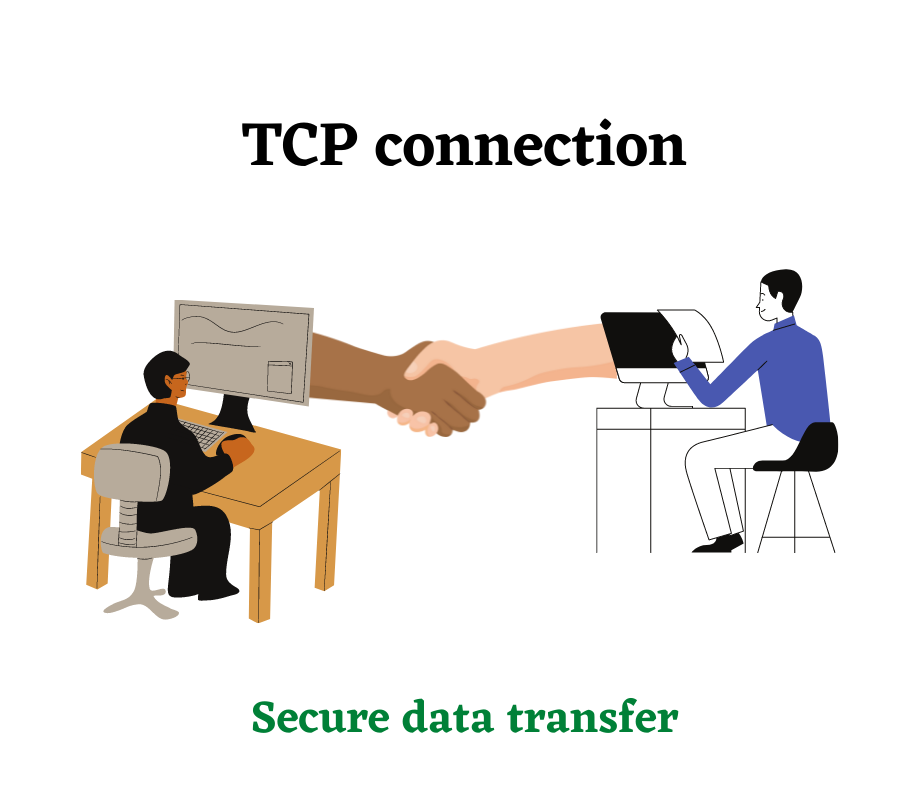
\includegraphics[scale=0.6]{content/chapter14/images/tcp.png}
		\caption{Secure TCP connection}
		\label{fig:tcp}
	\end{figure}

	\begin{itemize}
		\item TCP provides \textbf{reliable transmission, error control and in order} receiving of the data.
		\item Provides point to point connection.
		\item Eg : \textbf{Whatsapp, Instagram, Google Chat, Emails, browsing}
		\item Used when:
		\begin{itemize}
			\item Cannot tolerate the loss of data
			\item \textbf{Order} of data is importance
		\end{itemize}
	\end{itemize}
	
	\newpage
	\begin{figure}[h!]
		\centering
		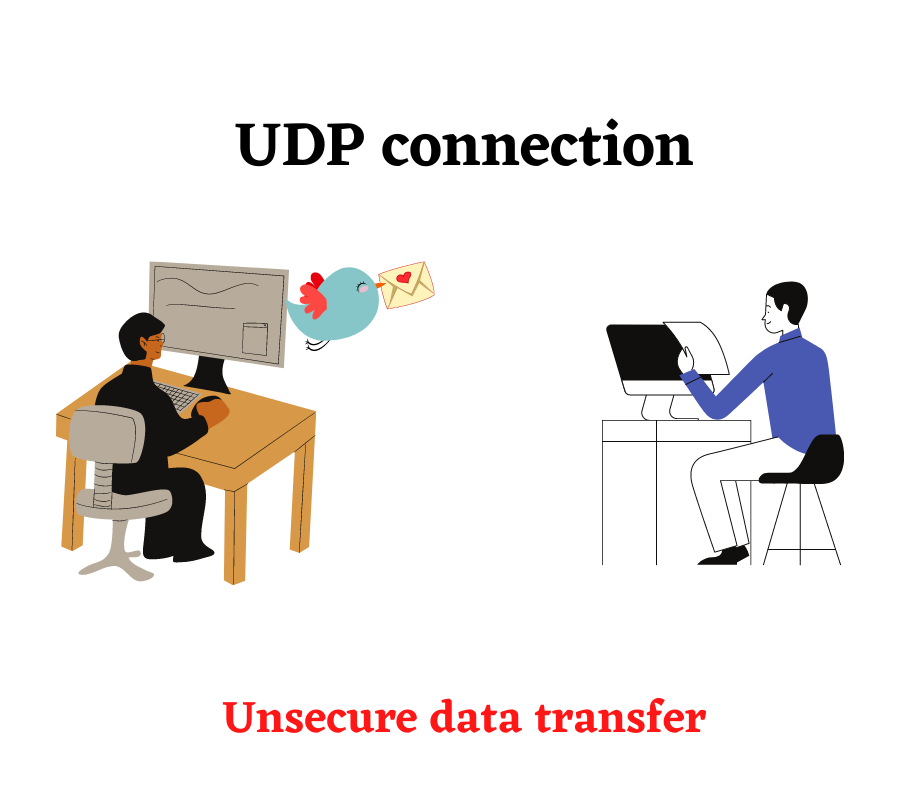
\includegraphics[scale=0.6]{content/chapter14/images/udp.png}
		\caption{Unsecure UDP connection}
		\label{fig:udp}
	\end{figure}
	
	\begin{itemize}
		\item UDP provides fast but \textbf{non-guaranteed transfer} of the data.
		\item No point to point connection.
		\item There is no connection establishment or termination on UDP.
		\item Eg: \textbf{Online gaming, Live streaming}

		
	\end{itemize}
	
	
	
	
	
\end{flushleft}
\newpage


